\documentclass{article}

% if you need to pass options to natbib, use, e.g.:
%     \PassOptionsToPackage{numbers, compress}{natbib}
% before loading neurips_2018

% ready for submission
% \usepackage{neurips_2018}

% to compile a preprint version, e.g., for submission to arXiv, add add the
% [preprint] option:
%     \usepackage[preprint]{neurips_2018}

% to compile a camera-ready version, add the [final] option, e.g.:
\usepackage[final]{projects}

% to avoid loading the natbib package, add option nonatbib:
%\usepackage[nonatbib]{neurips_2018}

\usepackage[utf8]{inputenc} % allow utf-8 input
\usepackage[T1]{fontenc}    % use 8-bit T1 fonts
\usepackage{hyperref}       % hyperlinks
\usepackage{url}            % simple URL typesetting
\usepackage{booktabs}       % professional-quality tables
\usepackage{amsfonts}       % blackboard math symbols
\usepackage{nicefrac}       % compact symbols for 1/2, etc.
\usepackage{microtype}      % microtypography
\usepackage{amsmath}
\usepackage{graphicx}
\usepackage{dsfont}
\usepackage{subcaption}
\usepackage{MnSymbol}%
\usepackage{wasysym}%

\usepackage{mathtools}

\usepackage[ruled]{algorithm2e}

\newtheorem{theorem}{Theorem}
\newtheorem{definition}{definition}
\newtheorem{lemma}{Lemma}
\newtheorem{proof}{Proof}[section]




\title{From Bound Majorization to Stochastic Bound Majorization}

\author{%
  Yunian Pan \\
  Department of Electrical Engineering \\ 
  \texttt{yp1170@nyu.edu} 
}

\begin{document}

\maketitle

\begin{abstract}
  Based on the bound majorization method for optimizing a partition function of log-linear models which uses a quadratic variational upper-bound to approximate the
  log-linear normalizer, outperforming state-of-the-art first- and second-order
  optimization methods on various learning tasks, a stochastic setting version of update was proposed in previous paper. The resulting stochastic second-order method
  outperforms stochastic gradient descent (across variations and various tunings) both in terms of the number of iterations and computation time till convergence
  while finding a better quality parameter setting. This report provides an empirical evaluation of this algorithm based on a simple multiclass logistic regression framework, 
  along with some additional proof of the convergence. 
\end{abstract}

\section{Introduction}

Estimation of the probability density function over sets of random variables is central to many learning problems. The estimation often requires optimization of the likelihood
of training datasets, which is the goal of logistic regression, CRF(conditional random fields) and many other log-linear models. This report will focus on a general
 partition function of such sort of log-linear models, discussing the majorization methods to optimize it. Then there will be some discussion about the convergence of both 
batch and stochastic setting. Finally a simple experiment of multiclass logistic regression based on the given optimization method will be presented.

 The main contents of this report will be organized as 3 parts:
 Section 2 presents the theoretical development of the algorithm and the stochastic version of it; Section 3 will give some analysis on the algorithms' convergence; Section 4
will give some empirical evaluation and comparisons under a multiclass logistic regression example.


\section{Theoretical development}

\subsection{partition function}

We begin our discussion from multinomial logistic regression, where we assume that the data are case specific, i.e. each independent variable has a single value for each case. 
The multinomial logistic model also assumes that the dependent variable cannot be perfectly predicted from the independent variables for any case.

The idea behind it, as in many other statistical classification techniques, is to construct a linear predictor function that constructs a score from a set of weights that
 are linearly combined with the explanatory variables (features) of a given observation using a dot product:
 \begin{equation}
  \begin{aligned}
   Score(x_i, k) = \theta_{k}^{\top } \cdot _i  \nonumber
  \end{aligned}
 \end{equation}
 where $x_i \in R^{d^{\prime}}$ is the vector of explanatory variables describing observation $i$, $\theta_k \in R^{d^{\prime}}$ is a vector of weights (or regression coefficients) corresponding to category $k \in \Omega$, and $Score(x_i, k)$
  is the score associated with assigning observation $i$ to category $k$. In discrete choice theory, where observations represent people and outcomes represent choices, the score is considered 
  the utility associated with person $i$ choosing outcome $k$. 
 The final predicted outcome is the one with the highest score.

 The difference between this type of setting and many other methods and algorithms such as SVM and perceptron etc. is the procedure for determining (training) the optimal coefficients
  and the way that the score is interpreted, the score can directly be converted to a probability value, indicating the probability of observation i choosing outcome k given the measured
   characteristics of the observation. 

   Then, we model the logarithm of the probability of seeing 
   a given output using the linear predictor as well as an additional normalization factor, the logarithm of the partition function:
   
    \begin{equation}
      \begin{aligned}
       &\ln \Pr(y_i | y_i = 1, x_i) = \theta_{1}^{\top } \cdot x_i - \ln Z  \nonumber \\
       &\ln \Pr(y_i | y_i = 2, x_i) = \theta_{2}^{\top } \cdot x_i - \ln Z  \nonumber \\
       &\ldots \ldots \ldots  \\ 
       &\ln \Pr(y_i | y_i = K, x_i) = \theta_{K}^{\top } \cdot x_i - \ln Z  \nonumber \\
      \end{aligned}
     \end{equation}
  
     We need an extra term $Z$ that has nothing to do with $y_i$ to ensure that $\sum_{k} h(y_i = k)\Pr(y_i | y_i=k, X_i) = 1$, (with the non-negative prior $h(y_i = k)$) 
     which is exactly the partition function of a simple conditional random field, this results in a soft-max function 
     $\Pr(y_i = n|x_i) = \frac{h(n)e^{\theta_n^{\top}x_i}}{\sum_{k}h(k) e^{\theta_k^{\top}x_i}}$.

     In a case that we don't want a set of different weights, we measure $\theta_k^{\top}x_i$ as $\theta^{\top}\textbf{f}_{x_i}(k)$, where $\textbf{f}: \Omega \to R^d$ is
     an arbitary mapping from the space of outcome to a real valued vector, $\theta^{\top}\in R^d$ is the coefficient that does not depend on the outcome.
     Thus we get rid of the index of parameter vector and develop a partition function that take in value of the single parameter vector, which is of the following
     form:
     \begin{equation}
      \begin{aligned}
       Z_{x_i}(\theta ) = \sum_{y \in \Omega} h(y) \exp(\theta^{\top} \textbf{f}_{x_i}(y)) 
      \end{aligned}
     \end{equation}    

For simplicity, the mapping we choose here is a filter that place the input $x_i$ on the position that corresponds to the choosing category/outcome, therefore $\theta$
can be viewed as a stack of the $k$ categories' parameter vectors, i.e. $\theta \in R^{kd^{\prime}}$. 

Note that the partition function also can arise naturally from the maximum entropy estimation or minimum relative entropy, or, KL divergence, $D(p\lVert h) = \sum_{y\in \Omega} p(y ) \log \frac{p(y)}{h(y)}$, 
where we estimate the distance from $p(y)$ seeing the prior $h(y)$.


\subsection{Upper bound of partition}

The partition function $Z(\theta) =  \sum_{y \in \Omega} h(y) \exp(\theta^{\top} \textbf{f}(y))$ will be the center of this section's analysis.
As the supplement of $^{[1]}$ provides, the first thing we do is reorder the outcome using a random mapping $\pi(\cdot): \Omega \to \{1,\ldots,n\} $,
s.t. $h(y) = h(\pi^{-1}(j)) = h_j$, $\textbf{f}(y) = \textbf{f}(\pi^{-1}(j)) = \textbf{f}_j$ and this is for explicity of the notation. Then we introduce a parameter $\lambda = \theta - \tilde{\theta}$,
and rewrite $Z(\theta) = \sum_{j=1}^{n} \alpha_j \exp(\lambda^{\top}\textbf{f}_j)$, where $\alpha_j = h(j) \exp(\tilde{\theta}^{\top}\textbf{f}_j)$.
In order to construct the monotonicity we denote $Z_i(\theta) = \sum_{j=1}^{i}\alpha_j \exp(\lambda^{\top}\textbf{f}_j)$, and a trivial bound holds for $i=0$:

\begin{equation}
  \begin{aligned}
   Z_{0}(\theta ) = 0 \leq z_0 \exp(\frac{1}{2} \bf{\lambda}^{\top} \Sigma_0 \lambda + \lambda^{\top} \bf{\mu}_0) 
  \end{aligned}
 \end{equation} 

 Here we set the parameters $z_0,\ \mu_0,\ \Sigma_0$ all close or equal to 0, with $z_0 = 0^{+},\ \mu_0 = \textbf{0},\ \Sigma_0 = z\bf{I}$ to make the bound tight.
 As we add another term $\alpha_1 \exp(\lambda^{\top} \bf{f}_1)$, on both side of the above inequality, the bound still holds, 
 \begin{equation}
  \begin{aligned}
   Z_{1}(\theta ) \leq z_0 \exp(\frac{1}{2} \bf{\lambda}^{\top} \Sigma_0 \lambda + \lambda^{\top} \mu_0) + \alpha_1 \exp(\lambda^{\top}\bf{f}_1) 
   \label{inequality2}
  \end{aligned}
 \end{equation} 

 Basically the idea is to transform the RHS of the inequality above to quadratic form so that 
 we can update the parameter $\Sigma_i$ and $\mu_i$ to $\Sigma_{i+1}$ and $\mu_{i+1}$ iteratively, ensuring that the final bound can be quadratic which is easy to optimize.
 For the convenience of observation we write the logarithm of $\ref{inequality2}$:

 \begin{equation}
  \begin{aligned}
   \log Z_{1}(\theta ) &\leq \log z_0 + \log (\exp(\frac{1}{2} \lambda^{\top} \Sigma_0 \lambda + \lambda^{\top} \mu_0) + \frac{\alpha_1}{z_0} \exp(\lambda^{\top}\textbf{f}_1)) \nonumber \\
    & = \log z_0 + \log (\exp(\frac{1}{2} \lambda^{\top} \Sigma_0 \lambda + \lambda^{\top} (\mu_0 - \textbf{f}_1)) + \frac{\alpha_1}{z_0} ) + \lambda^{\top}\textbf{f}_1  \nonumber \\
   \label{inequality3}
  \end{aligned}
 \end{equation}
 As we observed that it might be useful to seperate a term $\frac{1}{2}w^{\top}w = \frac{1}{2} (\textbf{f}_1 - \mu_0)^{\top} \Sigma_0^{-1} (\textbf{f}_1 - \mu_0)$ out of the log-exponential function
 such that the terms inside the logarithm can form a quadratic form $u^{\top} u = \frac{1}{2} (\textbf{f}_1 - \mu_0)^{\top} \Sigma_0^{-1} (\textbf{f}_1 - \mu_0) + \frac{1}{2} \lambda^{\top} \Sigma_0 \lambda + \lambda^{\top} \mu_0$, (there are still residual terms to dispose):
 \begin{equation}
  \begin{aligned}
   RHS & = \log z_0 +  \lambda^{\top}\textbf{f}_1 -\frac{1}{2}w^{\top}w + \log\exp \frac{1}{2}w^{\top}w \cdot (\exp(\frac{1}{2} \lambda^{\top} \Sigma_0 \lambda + \lambda^{\top} \mu_0) + \frac{\alpha_1}{z_0}) \\
       & = \log z_0 + \lambda^{\top}\textbf{f}_1 -\frac{1}{2}w^{\top}w + \log (\exp(\frac{1}{2} u^{\top} u) + \gamma)
  \label{inequality4}
  \end{aligned}
 \end{equation}
 where $\gamma = \frac{\alpha_1}{z_0} \exp \frac{1}{2}w^{\top}w$. Thus we are able to apply the lemma in $^{[3]}$ to bound the term $\log \exp(\frac{1}{2} u^{\top} u + \gamma)$.

 \begin{lemma}
  For all $u\in R^d$ and $v\in R^d$ and any $\gamma \geq 0$, the bound $\log(\exp(\frac{1}{2}\left\lVert u \right\lVert^2) + \gamma) \leq $
  \begin{equation}
    \log(\exp(\frac{1}{2}\left\lVert v \right\lVert^2) + \gamma) + \frac{ v^{\top} (u- v)}{1 + \gamma \exp(-\frac{1}{2}\left\lVert v \right\lVert^2)} + \frac{1}{2}(u-v)^{\top} (I + \Gamma vv^{\top})(u-v)         \nonumber
  \end{equation}
  holds when the scalar term $\Gamma = \frac{\tanh(\frac{1}{2}\log(\gamma \exp(-\frac{1}{2}\left\lVert v \right\lVert^2))}{2\log(\gamma \exp(-\frac{1}{2}\left\lVert v \right\lVert^2)}$, equality is achieved when $u = v$.
 \label{lemma1}
\end{lemma}

 Here we omit the proof of $\ref{lemma1}$. Apply the condition it provides that tightens the bound, $u = v$, by choosing $v = \Sigma_0^{-\frac{1}{2}}(\mu_0 - \textbf{f}_1)$,(after factorization,
 $u = \Sigma_0^{\frac{1}{2}} \lambda - \Sigma_0^{-\frac{1}{2}}(\mu_0 - \textbf{f}_1)$, and the inequality $\ref{inequality4}$ is achieved when $\lambda = 0$) 
 
 \begin{equation}
  \begin{aligned}
   \log Z_1(\theta) & \leq \log z_0 + \lambda^{\top}\textbf{f}_1 - \frac{1}{2} (\textbf{f}_1 - \mu_0)^{\top} \Sigma_0^{-1} (\textbf{f}_1 - \mu_0) \\
          & + \log(\exp(\frac{1}{2}\left\lVert v \right\lVert^2) + \gamma) + \frac{ v^{\top} (u- v)}{1 + \gamma \exp(-\frac{1}{2}\left\lVert v \right\lVert^2)} + \frac{1}{2}(u-v)^{\top} (I + \Gamma vv^{\top})(u-v)         \nonumber
       \label{inequality5}
  \end{aligned}
 \end{equation}
 
 Recall the previous attemption that transforming the RHS of the inequality to quadratic form:

 \begin{equation}
  \begin{aligned}
   Z_{1}(\theta )  \leq z_1 \exp(\frac{1}{2} \bf{\lambda}^{\top} \Sigma_1 \lambda + \lambda^{\top} \bf{\mu}_1) 
  \end{aligned}
 \end{equation} 

 Combined with $\ref{inequality5}$, using the method of undetermined coefficient, after some ugly algebra work we can solve for the equations and get the update:

 \begin{equation}
  \begin{aligned}
    z_1 &= z_0 + \alpha_1 \\ \nonumber 
    \mu_1 &=  \mu_0 + \frac{\alpha_1}{z_0 + \alpha_1} (\textbf{f}_1 - \mu_0) \\
    \Sigma_1 &= \Sigma_0 + \frac{\tanh(\frac{1}{2}\log(\nicefrac{\alpha_1}{z_0})}{2\log(\nicefrac{\alpha_1}{z_0})} (\textbf{f}_1 - \mu_0)(\textbf{f}_1 - \mu_0)^{\top}
     \end{aligned}
 \end{equation} 

 As we apply the procedure above successively until n, (assuming the cardinality $|\Omega| = n$ is finite and $\Omega$ is enumerable), the desired
 quadratic bound is achieved by mathematical induction.
 Equipped with the update equation above, Algorithm $\ref{algorithm1}$ can be proposed to compute the bound's parameters. It's notoriously that the log-expsum function
 is convex and the lower bound is given by Jensen's inequality, this algorithm contributes an analogous quadratic upper-bound on the partition function, as $\ref{bounds}$
 illustrated.

 \begin{algorithm}[H]
  \caption{Compute Bound}
  \KwIn{Parameters $\tilde{\theta},\ \textbf{f}(y),\ h(y)$}
  \textbf{Initialize:} $z \leftarrow 0^{+},\ \mu\leftarrow 0,\ \Sigma\leftarrow zI$\;    
  \For{ each $y\in \Omega$}{
    $\alpha = h(y)\exp(\tilde{\theta}^{\top}f(y))$ \\
    $\mu =  \mu + \frac{\alpha}{z+\alpha} (\textbf{f}(y) - \mu)$ \\
    $\Sigma = \Sigma + \frac{\tanh(\frac{1}{2}\log(\frac{\alpha}{z})}{2\log(\frac{\alpha}{z})} (\textbf{f}(y) - \mu)(\textbf{f}(y) - \mu)^{\top}$  \\
    $z = z + \alpha$  
    }
  \KwOut{$z$, $\mu$, $\Sigma$}
  \label{algorithm1}
  \end{algorithm}
  \begin{figure}
    \centering
    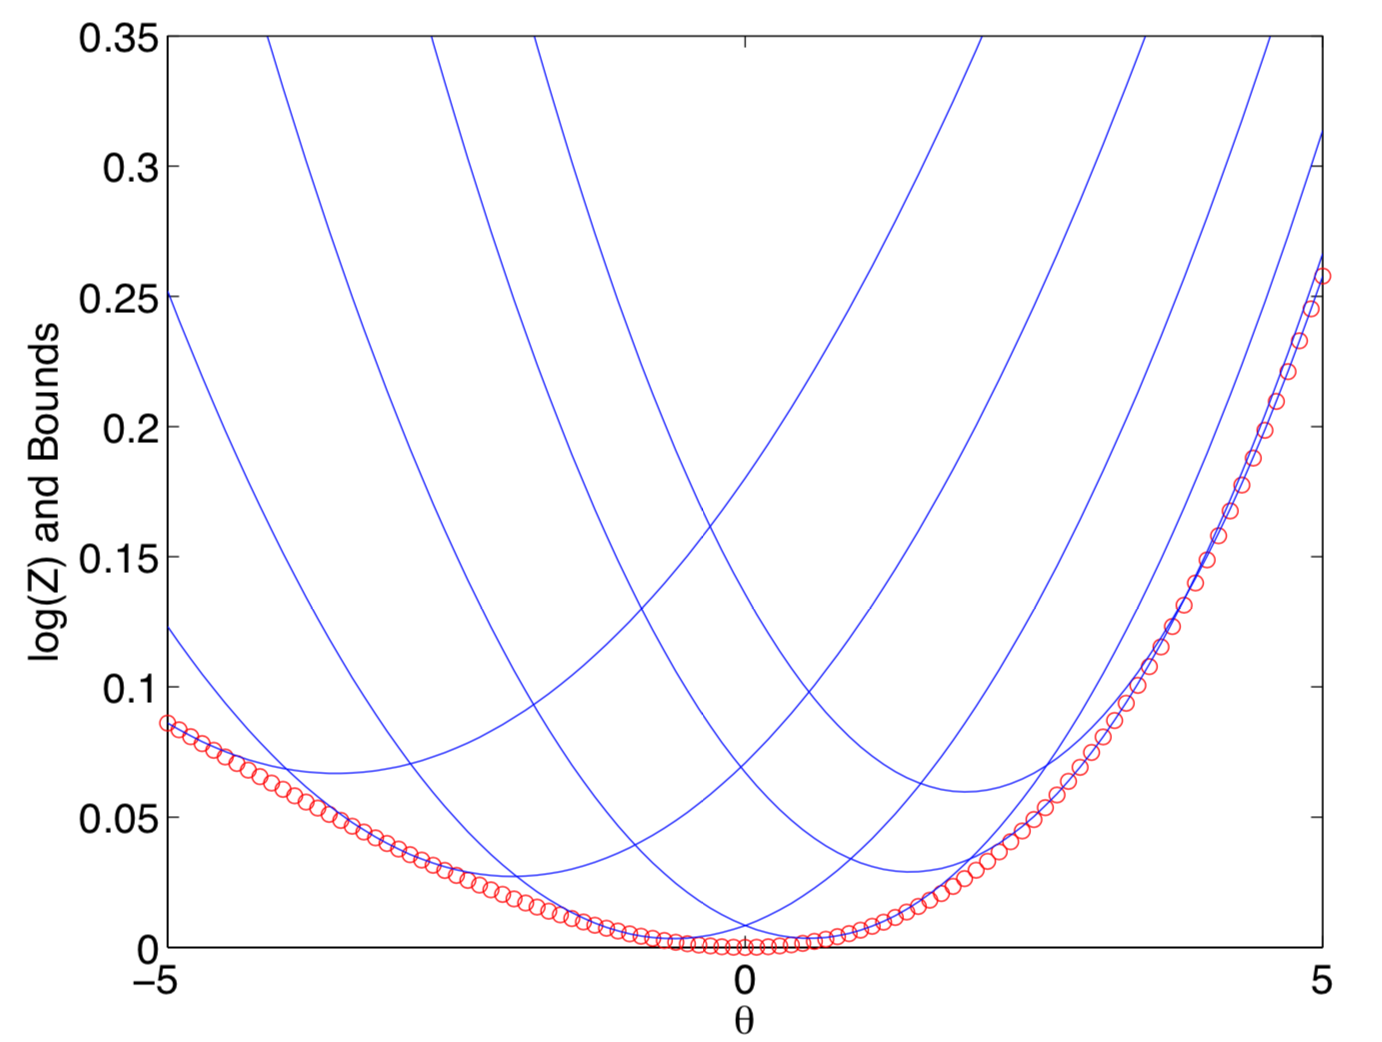
\includegraphics[width = .45\textwidth]{bound.png}
    \caption{bounds}
    \label{bounds}
  \end{figure}

\subsection{bound majorization}
Going back to the partition function, given a data-set ${(x_1, y_1), \ldots , (x_t, y_t)} $
of independent identically-distributed (i.i.d) input-output pairs where $y_i$ is the observed 
sample in a (discrete) space $\Omega_i$ conditioned on the observed input $x_i$, A CRF, or, let's say multinomial logistic regression's
parameter is estimated by maximizing the $l_2$ regularized loglikelihood of log-posterior: $\log \prod_{i=1}^{n}\Pr(y_i|x_i, \theta) - \frac{t\lambda}{2} \left\lVert\theta \right\lVert^2$,
where $\lambda \in R^+$ is a regularizing paramter to prevent the weights from exploding to infinity, we can write the total loglikelihood as follow:
\begin{equation}
  \begin{aligned}
   J(\theta ) = \sum_{i=1}^{t} [\log \frac{h_{x_i}(y_i)}{Z_{x_i}(\theta)} + \theta^{\top} \textbf{f}_{x_i}(y_i) - \frac{\lambda}{2} \left\lVert\theta \right\lVert^2 ]
  \end{aligned}
 \end{equation} 
 If prior knowledge (or constraints) restrict the solution vector to a convex hull $\Lambda$, the maximization
 problem becomes $ \arg \max_{\theta \in \Lambda} J (\theta)$, in practice we set $\Lambda \in R^d$. Recall the bound:
 
 \begin{equation}
  \begin{aligned}
   J(\theta ) & \geq \sum_{i=1}^{t} [\log h_{x_i}(y_i) - \log z_i  - \frac{1}{2} \bf{\lambda}^{\top} \Sigma_i \bf{\lambda} + \bf{\lambda}^{\top} \bf{\mu}_i + \theta^{\top} \textbf{f}_{x_i}(y_i) - \frac{\lambda}{2} \left\lVert \theta \right\lVert^2 ]    \\
 & = \sum_{i=1}^{t} [\log h_{x_i}(y_i) - \log z_i  - \frac{1}{2} (\theta - \tilde{\theta})^{\top} \Sigma_i (\theta - \tilde{\theta}) - (\theta - \tilde{\theta})^{\top} \bf{\mu}_i + \theta^{\top} \textbf{f}_{x_i}(y_i) - \frac{\lambda}{2} \left\lVert \theta \right\lVert^2 ] \\
 \end{aligned}
 \end{equation} 

As we drop the terms unrelated to $\theta$, the maximization problem becomes $\arg \min_{\theta} Q(\theta, \tilde{\theta})$, where:
\begin{equation}
  \begin{aligned}
    Q(\theta, \tilde{\theta}) &= \sum_i \frac{1}{2} (\theta - \tilde{\theta})^{\top}  \Sigma_i (\theta - \tilde{\theta}) + \theta ^{\top} \bf{\mu}_i - \theta^{\top} \textbf{f}_{x_i}(y_i) + \frac{\lambda}{2} \theta^{\top}\theta + \tilde{\theta}^{\top} \mu_i  ]   \\
  & = \sum_i \frac{1}{2} (\theta - \tilde{\theta})^{\top} \Sigma_i (\theta - \tilde{\theta}) +  \theta ^{\top} (\bf{\mu}_i - \textbf{f}_{x_i}(y_i)) + \frac{\lambda}{2} (\theta- \tilde{\theta})^{\top}(\theta- \tilde{\theta}) + \lambda\theta^{\top}\tilde{\theta} - \frac{\lambda}{2} \tilde{\theta}^{\top}\tilde{\theta} \\
 & =  \frac{1}{2} (\theta - \tilde{\theta})^{\top} (\sum_i (\Sigma_i + \lambda I) )(\theta - \tilde{\theta}) + \sum_i \theta ^{\top} (\bf{\mu}_i - \textbf{f}_{x_i}(y_i)+ \lambda \tilde{\theta}) - constant
\end{aligned}
 \end{equation} 

Thus resulting Algorithm 2, which has the similiar structure with EM algorithm, by constructing convex upper bound of the dual objective iteratively, hopefully we can
find the optimal solution of the original problem.

 \begin{algorithm}[H]
  \caption{BM}
  \KwIn{Input $x_i, y_i$ and functions $h_{x_i}, \textbf{f}_{x_i}$ for $i = 1,1, \ldots, t$, regularizer $\lambda \in R^+$ and convex hull $\Lambda \subseteq R^d$, $\epsilon$ }
  \textbf{Initialize:} $\theta_0$ anywhere inside $\Lambda$ and set $\tilde{\theta} = \theta_0$  \;    
  \While{ $\theta_{new} - \theta_{old} \geq \epsilon$}{
    \For{ $i = 1, \ldots, t$}{
      Get $\mu_i,\ \Sigma_i, $ from $h_{x_i},\ \textbf{f}_{x_i}, \tilde{\theta}$ via Algorithm 1
    }
    Set $\tilde{\theta} = \arg \min_{\theta} \frac{1}{2} (\theta - \tilde{\theta})^{\top} (\sum_{i} \Sigma_i + \lambda I)(\theta - \tilde{\theta}) + \theta^{\top} (\sum_{i} \mu_i - \textbf{f}_{x_i}(y_i) + \lambda \tilde{\theta})$ \\
Which means: $\tilde{\theta} = \tilde{\theta} - (\sum_i\Sigma + \lambda I)^{-1} (\sum_{i} \mu_i - \textbf{f}_{x_i}(y_i) + \lambda \tilde{\theta})$
    }
    
  \KwOut{$\hat{\theta} = \tilde{\theta}$}
  \label{algorithm2}
  \end{algorithm}

The proof of convergence under certain assumptions is given in $^{[1]}$ p.11, p.12, the basic idea is to construct an upper bound of the matrices $\Sigma_i$ and compare $J(\theta)$ to $J(\theta^*)$ for every iteration, which will be discussed in
the later section.

\subsection{Stochastic bound majorization}

The batch bound majorization algorithm assumes that we are in offline scenario where all the data are observable at once, $^{[2]}$ proposed a stochastic version of it,
which can be applied to online scenario.
\begin{algorithm}[H]
  \caption{Stochastic Bound Majorization}
  \KwIn{prior $h(\cdot)$, function $\textbf{f}(\cdot)$, regularizer $\lambda \in R^+$ and convex hull $\Lambda \subseteq R^d$ $\epsilon$}
  \textbf{Initialize:} $\theta_0$ anywhere inside $\Lambda$ and set $\tilde{\theta} = \theta_0$  \;    
  \While{ $\theta_{new} - \theta_{old} \geq \epsilon$}{
    randomly select $p$ mini-batch $x_i, y_i$'s \\
    \For{ $i = 1, \ldots, p$}{
      Get $\mu_i,\ \Sigma_i, $ from $h_{x_i},\ \textbf{f}_{x_i}, \tilde{\theta}$ via Algorithm 1
    }
    Set $\tilde{\theta} = \arg \min_{\theta} \frac{1}{2} (\theta - \tilde{\theta})^{\top} (\sum_{i} \Sigma_i + \lambda I)(\theta - \tilde{\theta}) + \theta^{\top} (\sum_{i} \mu_i - \textbf{f}_{x_i}(y_i) + \lambda \tilde{\theta})$ \\
Which means: $\tilde{\theta} = \tilde{\theta} - (\sum_i\Sigma + \lambda I)^{-1} (\sum_{i} \mu_i - \textbf{f}_{x_i}(y_i) + \lambda \tilde{\theta})$
    }
    
  \KwOut{$\hat{\theta} = \tilde{\theta}$}
  \label{algorithm3}
  \end{algorithm}

There are also a variation of this algorithm, as we notice that the update of $\theta$ can be viewed as a linear system:

\begin{equation}
  \begin{aligned}
    (\sum_j \Sigma_{j}(\theta_{n-1}) + \lambda I) (\theta_n - \theta_{n-1}) = \sum_{j} \mu_j(\theta_{n-1})
  \end{aligned}
 \end{equation} 

 Where we can write $(\sum_j \Sigma_{j}(\theta_{n-1}) + \lambda I)^{-1}$ as $M$ and apply the Sherman-Morrison formula $(\Sigma + (\sqrt{\beta}l)^{\top}(\sqrt{\beta}l))^{-1} = \Sigma^{-1} - \frac{\Sigma^{-1} (\sqrt{\beta}l)^{\top}(\sqrt{\beta}l)\Sigma^{-1}}{1 + (\sqrt{\beta}l)^{\top} \Sigma^{-1} (\sqrt{\beta}l)}$,
 where the term $\beta = \frac{\tanh(\frac{1}{2}\log(\frac{\alpha}{z})}{2\log(\frac{\alpha}{z})}$, $l = \textbf{f}(y) - \mu$, thus rewrite the update formula of $\Sigma_i$ as:
 \begin{equation}
  \begin{aligned}
    M_{n+1} = M_{n} - \frac{\beta M_n l^{\top} l M_n}{1 + \beta l^{\top} M_n l}
  \end{aligned}
  \label{sherman}
 \end{equation} 

 $\ref{sherman}$ can be incorporated to the reformulation of $\theta$ update, specifically, during period of one-time update over a mini-batch dataset of size $t$ we update the matrix $M$ and $\mu$ $T = nt$ times, and we can expand
 $\phi = M_{T} \mu_{T}$ successively $T$ times until $M_0,\ \mu_0$:
 \begin{equation}
  \begin{aligned}
    \theta & = \theta - \eta M_T \mu_T \nonumber \\
    & = \theta - \eta ( M_{T-1} \mu_{T-1} + M_{T}(\kappa_{T-1} l_{T-1} - \text{f}_{T-1} + \frac{\lambda \theta}{t})  - \frac{\beta_{T-1} M_{T-1} l_{T-1}^{\top} l_{T-1} M_{T-1}}{1 + \beta_{T-1} l_{T-1}^{\top} M_{T-1} l_{T-1}} \mu_{T-1} ) \\
    & \cdots \cdots \\
    & = \theta - \eta(M_0 \mu_0 + \sum_{i=0}^{T-1} M_{i}(\kappa_{i-1} l_{i-1} - \text{f}_{i-1} + \frac{\lambda \theta}{t}) - \frac{\beta_{i-1} M_{i-1} l_{i-1}^{\top} l_{i-1} M_{i-1}}{1 + \beta_{i-1} l_{i-1}^{\top} M_{i-1} l_{i-1}} \mu_{i-1} ) 
  \end{aligned}
  \label{shermanupdate}
 \end{equation} 

 Leveraging the equation above, algorithm $\ref{algorithm4}$ was proposed as we can adjust the algorithm by terminating the summation before the $\theta$ is allowed to update, i.e. analogous to SGD,
 the most natural way to convert batch setting algorithm to mini-batch setting is to interleave updates of the parameter $\theta$, the update rule will be given as:
 \begin{equation}
  \begin{aligned}
    \theta_{i+1} = \theta_i - \eta( \sum_{y =1}^{n} M_{i}(\theta_i)(\kappa_i(\theta_i) l_i(\theta_i) - \text{f}_i(\theta_i) + \frac{\lambda \theta_i}{t}) - \frac{\beta_i M_i(\theta_i) l_i(\theta_i)^{\top} l_{i}(\theta_i) M_{i}(\theta_i)}{1 + \beta_{i}(\theta_i) l_{i-1}(\theta_i)^{\top} M_{i}(\theta_i) l_{i}(\theta_i)} \mu_{i}(\theta_i) )  \nonumber
  \end{aligned}
  \label{updaterule}
 \end{equation} 
 Note that the rule above is for one data point, the update rule also admits mini-batch. The algorithm, which performs a full-rank update of $\Sigma$, again can be adjusted to low-rank version.
  
 \begin{algorithm}[H]
    \caption{SBM}
    \KwIn{prior $h(\cdot)$, function $\textbf{f}(\cdot)$, regularizer $\lambda \in R^+$ and convex hull $\Lambda \subseteq R^d$ , step size $\eta$, $\epsilon $}
    \textbf{Initialize:} $\theta_0$ anywhere inside $\Lambda$ and set $\tilde{\theta} = \theta_0$,  $\phi = \textbf{0}$,  $M = \frac{1}{\lambda} I$,  $\mu = 0$\;    
    \While{ $\theta_{new} - \theta_{old} \geq \epsilon$}{
      randomly select $p$ mini-batch $x_i, y_i$'s \\
      \For{ $i = 1, \ldots, p$}{
        $z \leftarrow 0^+$; $g = 0$ \\
        \For{each $y \in \Omega$} {
        $\alpha = h(y)\exp(\tilde{\theta}^{\top}f(y))$   $\quad l = f(y) - g$ $\quad \beta = \frac{\tanh(\frac{1}{2}\log(\frac{\alpha}{z})}{2\log(\frac{\alpha}{z})}$  $\quad z = z + \alpha$   $\quad \kappa = \frac{\alpha}{z}$ \\   
        $M = M - \frac{\beta M l^{\top} l M}{1 + \beta l^{\top} M l}$ \\
        $\phi = \phi + M (\kappa l - \text{f}_{x_i}(y) + \frac{\lambda \tilde{\theta}}{t}) -\frac{\beta M l^{\top} l M}{1 + \beta l^{\top} M l} \mu $ \\
        $\mu = \mu + \kappa l - \text{f}_{x_i}(y) + \frac{\lambda \tilde{\theta}}{t}$ \\
        $g = g + \kappa l$
        } 
       
       }$\tilde{\theta} = \tilde{\theta} - \eta \phi $
      }   
    \KwOut{$\hat{\theta} = \tilde{\theta}$}
    \label{algorithm4}
    \end{algorithm}


\section{Discussion of the convergence}

\subsection{upper bound of batch setting convergence rate}

We begin by comparing two functions' supremums, at each iteration there will be a slight change on matrix $\Sigma$,there's a lemma which would be useful
for quantitatively measuring the difference of each iteration.

\begin{lemma}
 If $\kappa \Psi \succeq \Phi$ for $\Psi \succeq \Phi \in R^{d \times d}$, then
\begin{equation}
  \begin{aligned}
  L(\theta ) = -\frac{1}{2}(\theta  - \tilde{\theta})^{\top} \Phi (\theta  - \tilde{\theta}) - (\theta  - \tilde{\theta})^{\top}\mu \\ \nonumber
  U(\theta) = -\frac{1}{2}(\theta  - \tilde{\theta})^{\top} \Psi (\theta  - \tilde{\theta}) - (\theta  - \tilde{\theta})^{\top}\mu 
 \end{aligned}
 \end{equation}
  satisfy $\sup_{\theta \in \Lambda} U(\theta)$ for any convex $\Lambda \subseteq R^d, \ \tilde{\theta} \in  \Lambda, \ \mu \in R^d$ and $\kappa \in R^+$ 
\label{dual}
\end{lemma}

The basic idea to prove this lemma is to find the relationship between the dual problems. Leveraging this lemma, first we upper-bound the matrix
$\Sigma_i$ by assuming $\left\lVert \textbf{f}_{x_i}(y) \right\lVert^2 \leq r^2 \ \ \forall y\in \Omega $ and since $\mu_i$ is a convex combination of $\textbf{f}_{x_i}(y)$,
the outer-product terms in the update for $\Sigma_i$ satisfy:
\begin{equation}
  (\textbf{f}_{x_i}(y) - \mu_i)(\textbf{f}_{x_i}(y) - \mu_i)^{\top} \preceq 4r^2 I \nonumber
\end{equation}

Thus $\Sigma_i \preceq \mathcal{F}(\alpha_1, \ldots, \alpha_n) 4r^2 I$ holds, where
\begin{equation}
  \mathcal{F}(\alpha_1, \ldots, \alpha_n) =\sum_{i=2}^{n} \frac{\tanh(\frac{1}{2} \log(\frac{\alpha_i}{\sum_{k=1}^{i-1} \alpha_k}))}{2 \log (\frac{\alpha_i}{\sum_{k=1}^{i-1} \alpha_k})} \nonumber
\end{equation}
$\alpha_1, \ldots, \alpha_n$ are defined in the algorithm 1, the formula for $\mathcal{F}$ starts at $i = 2$ since initialization. Assuming the permutation $\pi$ is sampled uniformly at random,
the expectation of $\mathcal{F}$ will be:
\begin{equation}
  E_{\pi}[\mathcal{F}(\alpha_1, \ldots, \alpha_n)] = \frac{1}{n!}\sum_{\pi}\sum_{i=2}^{n} \frac{\tanh(\frac{1}{2} \log(\frac{\alpha_{\pi(i)}}{\sum_{k=1}^{i-1} \alpha_{\pi(k)}}))}{2 \log (\frac{\alpha_{\pi(i)}}{\sum_{k=1}^{i-1} \alpha_{\pi(k)}})} \nonumber
\end{equation}

Analyzing this function can be daunting as the derivative is complicated, at the very first we guess that the expectation will be maximized when all $\alpha_i$'s are the same, then we observe that due to expectation, $\frac{\partial E}{\partial \alpha_i} = \frac{\partial E}{\partial \alpha_j} \ \ \forall i,j$,
and $\mathcal{F}$ is invariant to any scaling of all $\alpha_i$'s, so the gradient $ \nabla_{\alpha} E_{\pi}(\mathcal{F})_{ |\alpha_i = constant}$ must be all 0, therefore
any point $\alpha_i = constant$ will be either an extremum or a saddle point. Then we consider $\frac{\partial^2 \mathcal{F}}{\partial \alpha_i^2}$ and $\frac{\partial^2 \mathcal{F}}{\partial \alpha_i \partial \alpha_j}$, 

\begin{equation}
  \begin{aligned}
    \frac{\partial^2 \mathcal{F}}{\partial \alpha_i^2} &= \frac{\partial^2 f(\frac{\alpha_i}{\alpha_{i-1}+ \ldots})}{\partial \alpha_i^2} + \frac{\partial^2 f(\frac{\alpha_{i+1}}{\alpha_{i}+ \ldots})}{\partial \alpha_i^2} + \ldots \nonumber  \\ 
    \frac{\partial^2 \mathcal{F}}{\partial \alpha_i \partial \alpha_j} &= \frac{\partial^2 f(\frac{\alpha_j}{\alpha_{j-1}+ \ldots})}{\partial \alpha_i\partial \alpha_j} + \frac{\partial^2 f(\frac{\alpha_{j+1}}{\alpha_{j}+ \ldots})}{\partial \alpha_i \partial \alpha_j} + \ldots (j > i)\\
    \frac{\partial^2 \mathcal{F}}{\partial \alpha_i \partial \alpha_j} &= \frac{\partial^2 f(\frac{\alpha_i}{\alpha_{i-1}+ \ldots})}{\partial \alpha_i\partial \alpha_j} + \frac{\partial^2 f(\frac{\alpha_{i+1}}{\alpha_{j}+ \ldots})}{\partial \alpha_i \partial \alpha_j} + \ldots (j < i) 
  \end{aligned}
\end{equation}

where $f(\frac{\alpha_i}{\alpha_{i-1}+ \ldots}) = \frac{\tanh(\frac{1}{2} \log(\frac{\alpha_{\pi(i)}}{\sum_{k=1}^{i-1} \alpha_{\pi(k)}}))}{2 \log (\frac{\alpha_{\pi(i)}}{\sum_{k=1}^{i-1} \alpha_{\pi(k)}})}$. It's obvious to notice that $\frac{\partial^2 \mathcal{F}}{\partial \alpha_i \partial \alpha_j}$ is either of the same form with $\frac{\partial^2 \mathcal{F}}{\partial \alpha_i^2}$ or be part of it
when $\alpha_i = \alpha_j$, therefore once the terms in $\frac{\partial^2 \mathcal{F}}{\partial \alpha_i^2}$
is determined, so is $\frac{\partial^2 \mathcal{F}}{\partial \alpha_i \partial \alpha_j}$. Essentially, $\frac{\partial^2 E}{\partial \alpha_i \partial \alpha_j} = -\frac{1}{n-1}\frac{\partial^2 E}{\partial \alpha_i^2} $ while
$\frac{\partial^2 E}{\partial \alpha_i^2}$ is negative thus $\alpha_i = constant$ is locally concave and 
yeilds the Loewner ordering sense upper bound:

\begin{equation}
  \Sigma_i \preceq (2 r^2 \sum_{i=2}^{n} \frac{\tanh(\frac{1}{2}\log i)}{\log i} )I = \omega I
 \end{equation}

 Equipped with this bound, it's natural to rewrite the $L(\theta)$ and $U(\theta)$ in $\ref{dual}$ as:
 \begin{equation}
  \begin{aligned}
     J(\theta)  &\geq J(\tilde{\theta})-\frac{1}{2}(\theta - \tilde{\theta})^{\top} (\sum_i^t \Sigma_i + t\lambda I )(\theta - \tilde{\theta}) - (\theta - \tilde{\theta})^{\top}\mu \\ & =  L(\theta ) \\
    J(\theta)  &\leq J(\tilde{\theta})-\frac{1}{2}(\theta - \tilde{\theta})^{\top} ( t\lambda I )(\theta - \tilde{\theta}) - (\theta - \tilde{\theta})^{\top} \mu \\ & =  U(\theta )
  \end{aligned}
\end{equation}

At time $\tau $ after some iterations of traverse through the data, suppose we get the loglikelihood $J(\theta_{\tau}) = J(\tilde{\theta})$, it's clearly that it's bounded by lower bound $L_{\tau}(\theta)$ and upper bound $U_{\tau}(\theta)$ and
only when $\theta = \theta_{\tau}$ the equality $L_{\tau}(\theta) = J_{\tau}(\theta) =U_{\tau}(\theta)$ holds, in the next epoch the 
procedure is to set $\theta_{\tau+1} = \arg \min_{\theta \in \Lambda} J_{\tau}(\theta)$, but in the context of lower bound where we replace $\Sigma$ with $\omega I$,
it makes less progress when setting $\theta_{\tau+1} = \arg \min_{\theta \in \Lambda} L_{\tau}(\theta)$, which means $J(\theta_{\tau+1}) \geq \sup_{\theta \in \Lambda}L_{\tau}(\theta)$, setting $\Psi = t\lambda I$, $\Phi = (tw+ t\lambda)I$ and $\kappa = \frac{w + \lambda}{\lambda}$, apply lemma $\ref{dual}$:

\begin{equation}
  \sup_{\theta \in \Lambda} L_{\tau}(\theta) - L_{\tau}(\theta_{\tau}) = \frac{1}{\kappa} \sup_{\theta \in \Lambda} U_{\tau}(\theta) - U_{\tau}(\theta_{\tau}) \nonumber
 \end{equation}

 It's trivial that $J(\theta^{*}) \leq sup_{\theta \in \Lambda}U_{\tau}(\theta)$, thus:
 \begin{equation}
  \begin{aligned}
    J(\theta_{\tau+1}) - J(\theta_{\tau}) &\geq \frac{1}{\kappa}(J(\theta^*) - J(\theta_{\tau})) \\
   \implies J(\theta_{\tau+1}) - J(\theta^*) &\geq (1-\frac{1}{\kappa})(J(\theta_{\tau}) - J(\theta^*))   \nonumber
  \end{aligned}
 \end{equation}

 successively,
\begin{equation}
  J(\theta_{\tau}) - J(\theta^*) \geq (1-\frac{1}{\kappa})^{\tau}(J(\theta_{0}) - J(\theta^*))  
  \label{iterations}
\end{equation}

Therefore if we want $J(\theta_{\tau}) - J(\theta_{\tau}) \leq \epsilon(J(\theta^*) - J(\theta_{\tau}))$ we need more than $\tau = [\frac{\log(\epsilon)}{\log(\kappa-1) - \log \kappa}]$ epochs
of training. Note that here no guarantee of convergence is provided, $\ref{iterations}$ only provided a estimation of how far we have to go in order to obtain the desired optimal.




\subsection{Convergence guarantee of batch bound majorization}

%We started from stochastic version as once the convergence is proved for online case, it holds the same for offline case as they are all
%sample-based, we can average the loglikelihood without affecting the updating rule. 
Define mapping: $G(\theta) \coloneqq \theta - \eta V(\theta )$
where $V(\theta) = \Sigma^{-1}(\theta) \mu(\theta)$, our effort is equivalent to finding the solution to the fixed point equation: $\theta^* = G(\theta^*)$,
which simply indicates: $\Sigma^{-1}(\theta^*) \mu(\theta^*) = 0$. (Following convexity we know that $\theta^*$'s existence and uniqueness.)

Begin with an initialization $\theta_0$ that is close enough to the optimal $\theta^*$, $\left\lVert\theta_0 - \theta^*\right\lVert_2^2 \leq \frac{d}{2}$.
Since $Q(\cdot| \theta)$ is a quadratic function that has very nice properties, one can pick some $\epsilon$ and $l$ s.t $Q(\cdot| \theta)$ is both $\epsilon$ strongly convex and $l$ smooth.
and since the minimization of $Q$ is within some convex hull $\Lambda$, or, let's say an Euclidean ball $B(\frac{d}{2}, \theta_0)$, thus all iterates reamain within
an d-ball of $\theta^*$.

Following a standard result from the optimization theory, we further propose lemma $\ref{contractive}$:
\begin{lemma}
  Define a mapping $L(\theta) \coloneqq \theta - \eta V(\theta^*) $ which is equivalent to appling gradient operator $T(\theta)\coloneqq \theta - \eta \nabla Q(\theta|\theta^*)$ $z_{\theta}$ times, i.e. $L(\theta) = T^{z_{\theta}}(\theta)$, where $z_{\theta}$ is a finte integer, and $\nabla Q(\theta|\theta^*)$  is the gradient w.r.t population, under strong
  convexity condition and smoothness assumption which already hold with stepsize $\eta = \frac{2}{\epsilon+l}$, and because $T(\theta)$ is contractive, we have:
  \begin{equation}
    \left\lVert L(\theta) - \theta^* \right\lVert_2 \leq (\frac{l - \epsilon}{l+ \epsilon})^{z_{\theta}}\left\lVert \theta - \theta^* \right\lVert_2
  \label{contraction}
  \end{equation} 
  \label{contractive}
\end{lemma}
Here we leverage several truths as follows to recursively find the inequality:
\begin{itemize}
  \item The standard result $ \left\lVert T(\theta) - \theta^* \right\lVert_2 \leq (\frac{l - \epsilon}{l+ \epsilon})\left\lVert \theta - \theta^* \right\lVert_2  $ 
  \item $z_{\theta}$ is the number of iteration that we perform to optimize a quadratic problem which is theoretically finite.
  \item $ T^{z_{\theta}}(\theta_{z_{\theta}}) = T T^{z_{\theta}-1}(\theta_{z_{\theta}-1})$
\end{itemize}

Therefore we are able to focus on the update:

\begin{equation}
  \begin{aligned}
    \left\lVert G(\theta) - \theta^* \right\lVert_2 & = \left\lVert \theta - \eta V(\theta)- \theta^* \right\lVert_2 \nonumber \\
    & \leq \left\lVert \theta - \eta V(\theta^*)- \theta^* \right\lVert_2 + \eta \left\lVert  V(\theta)-V(\theta^*) \right\lVert_2 \\
    & = \left\lVert L(\theta)- \theta^* \right\lVert_2 + \eta \left\lVert  V(\theta)-V(\theta^*) \right\lVert_2 
  \end{aligned}
 \end{equation}

Notice that we have to make another assumption that the term $\left\lVert  V(\theta)-V(\theta^*) \right\lVert$ is stablized by 
the distance $\left\lVert \theta - \theta^* \right\lVert_2$ in order to prove the convergence. Analogous to the gradient stability
condition, it's natural to come up with the assumption $\ref{Vstable}$:

\begin{definition}{$V(\theta)$ stability}

  The functions $\{Q(\cdot|\theta), \theta \in \Omega\}$ statisfy VS($\gamma$) condition, where $\gamma \geq 0$, over Euclidean ball $B_2(d, \theta^*)$,
  if 
  \begin{equation}
     \left\lVert\Sigma(\theta)^{-1}\mu(\theta) - \Sigma(\theta^*)^{-1}\mu(\theta^*)\right\lVert_2 \leq \gamma  \left\lVert \theta - \theta^*\right\lVert_2
  \end{equation}
  for all $\theta \in B_2(d, \theta^*)$
  \label{Vstable}
\end{definition}

Therefore, going back to the update rule:
\begin{equation}
  \begin{aligned}
    \left\lVert G(\theta) - \theta^* \right\lVert_2  \leq ((\frac{l - \epsilon}{l+\epsilon} )^{z(\theta)} + \eta \gamma)\left\lVert \theta - \theta^* \right\lVert_2 
  \end{aligned}
 \end{equation}

Thus result in $ \left\lVert \theta_n - \theta^* \right\lVert_2  \leq ((\frac{l - \epsilon}{l+\epsilon} )^{z(\theta)} + \eta \gamma)^n \left\lVert \theta_0 - \theta^* \right\lVert $. Since $\frac{l-\epsilon}{l+\epsilon} > (\frac{l-\epsilon}{l+\epsilon})^{z_{\theta}}$,
we only need to ponder whether $(\frac{l - \epsilon}{l+\epsilon} ) + \eta \gamma < 1$ or not, which obviously holds when we have $\epsilon > \gamma$ (we've already set $\eta = \frac{2}{l+\epsilon}$), thus ensuring the term $(\frac{l - \epsilon}{l+\epsilon} )^{z(\theta)} + \eta \gamma < 1$  
along with the convergence of the update. 

\subsection{Convergence guarantee of stochastic bound majorization}

Note that this is actually a Robbins Monro problem, where we define stepsize $\eta_t$ of order $O(\frac{1}{n})$ to ensure that $\sum \eta_t = \infty$ and $\sum \eta_t^2 <\infty $, note that the updating rule
in stochastic version becomes $G(\theta):= \theta - \eta \hat{V}(\theta)$, where $\hat{V}(\theta)$ is related to the randomly sampled mini-batch.
At the very first beginning let's introduce several machineries. For a wider range of step sizes, lemma $\ref{contractive3}$ holds that

\begin{lemma}
  Define a mapping $L(\theta) \coloneqq \theta - \eta V(\theta^*) $ which is equivalent to appling gradient operator $T(\theta)\coloneqq \theta - \eta \nabla Q(\theta|\theta^*)$ $z_{\theta}$ times, i.e. $L(\theta) = T^{z_{\theta}}(\theta)$, where $z_{\theta}$ is a finte integer, and $\nabla Q(\theta|\theta^*)$  is the gradient w.r.t population, under strong
  convexity condition and smoothness assumption which already hold with stepsize $0 \leq \eta \leq \frac{2}{\epsilon+l}$, and because $T(\theta)$ is contractive, we have:
  \begin{equation}
    \left\lVert L(\theta) - \theta^* \right\lVert_2 \leq (1 - \frac{2\eta l \epsilon}{l+ \epsilon})^{z_{\theta}}\left\lVert \theta - \theta^* \right\lVert_2
  \label{contraction}
  \end{equation} 
  \label{contractive3}
\end{lemma}

Similarly using the exactly the same technique as before we can get:
\begin{equation}
  \begin{aligned}
    \left\lVert G(\theta) - \theta^* \right\lVert_2  \leq ((1 - \frac{2\eta l \epsilon}{l+ \epsilon})^{z_{\theta}} + \eta \gamma)\left\lVert \theta - \theta^* \right\lVert_2
  \end{aligned}
 \end{equation}

 Therefore we are done preparing for all the mathematical machineries to prove the convergence guarantee. Denote $\Delta_{t+1}:= \theta_{t+1} - \theta^*$, we have that:
 \begin{equation}
   \begin{aligned}
     \left\lVert\Delta_{t+1}\right\lVert_2^2 - \left\lVert\Delta_{t}\right\lVert_2^2 & \leq (\eta_t)^2 \left\lVert\hat{V}(\theta_{t})\right\lVert_2^2 + 2\eta_t \left\lVert\hat{V}(\theta_{t}) \cdot \Delta_t \right\lVert_2 \\ \nonumber
   \implies E[ \left\lVert\Delta_{t+1}\right\lVert_2^2 ] & \leq E[\left\lVert\Delta_{t}\right\lVert_2^2] + (\eta_t)^2 E[\left\lVert\hat{V}(\theta_{t})\right\lVert_2^2] + 2\eta_t E[\left\lVert\hat{V}(\theta_{t}) \cdot \Delta_t \right\lVert_2 ]
    \end{aligned}
  \end{equation}

  Since $\hat{V}(\theta^*) = 0$, we have:
  \begin{equation}
    \begin{aligned}
    E[ \left\lVert\Delta_{t+1}\right\lVert_2^2 ] & \leq E[\left\lVert\Delta_{t}\right\lVert_2^2] + (\eta_t)^2 E[\left\lVert\hat{V}(\theta_{t})\right\lVert_2^2] + 2\eta_t E[\left\lVert(\hat{V}(\theta_{t}) -\hat{V}(\theta^*) )  \cdot \Delta_t \right\lVert_2 ]  \nonumber
     \end{aligned}
   \end{equation}

  Then we upper bound the last term using $(\left\lVert G(\theta) - \theta^*\right\lVert_2 \leq (1 - \frac{2\eta l \epsilon}{l+ \epsilon})^{z_{\theta}} + \eta \gamma)\left\lVert \theta - \theta^* \right\lVert_2$, which is: $2\eta_t E[\left\lVert(\hat{V}(\theta_{t}) -\hat{V}(\theta^*) )  \cdot \Delta_t \right\lVert_2 \leq (1 - \frac{2\eta l \epsilon}{l+ \epsilon})^{z_{\theta}} + \eta \gamma -1 )\left\lVert \theta_t - \theta^* \right\lVert_2$
and we get:
\begin{equation}
  \begin{aligned}
  E[ \left\lVert\Delta_{t+1}\right\lVert_2^2 ] & \leq E[\left\lVert\Delta_{t}\right\lVert_2^2] + (\eta_t)^2 E[\left\lVert\hat{V}(\theta_{t})\right\lVert_2^2] - 2((1 - \frac{2\eta_t l \epsilon}{l+ \epsilon})^{z_{\theta}} + \eta_t \gamma -1 )E[\left\lVert\Delta_t \right\lVert_2^2]  \nonumber
   \end{aligned}
 \end{equation}

For simplicity it's safe to set $z(\theta) = 1$ as the inequality still holds and we get: 
\begin{equation}
  \begin{aligned}
  E[ \left\lVert\Delta_{t+1}\right\lVert_2^2 ] & \leq E[\left\lVert\Delta_{t}\right\lVert_2^2] + (\eta_t)^2 E[\left\lVert\hat{V}(\theta_{t})\right\lVert_2^2] - 2\eta_t \xi E[\left\lVert\Delta_t \right\lVert_2^2]  \nonumber
   \end{aligned}
 \end{equation}
where $\xi = \frac{2l\epsilon}{l+\epsilon} - \gamma$, combining all the previous results and upper bounding the second term $\sup_{\theta \in \Lambda}E[\left\lVert\hat{V}(\theta_{t})\right\lVert_2^2] = \sigma_{V}^2$:
\begin{equation}
  \begin{aligned}
  E[ \left\lVert\Delta_{t+1}\right\lVert_2^2 ] & \leq (1 - 2\eta_t \xi)E[\left\lVert\Delta_{t}\right\lVert_2^2] + (\eta_t)^2 E[\left\lVert\hat{V}(\theta_{t})\right\lVert_2^2] \nonumber \\
& \leq   (1 - \eta_t \xi)E[\left\lVert\Delta_{t}\right\lVert_2^2] + (\eta_t)^2 \sigma_{V}^2 \nonumber 
  \end{aligned}
\end{equation}
Setting $\eta_t =\frac{3}{2\xi(t+2)}$ and nwrapping the recursion, after some algebra work including summation, multiplication, contraction and upper bounding,
\begin{equation}
  \begin{aligned}
  E[ \left\lVert\Delta_{t+1}\right\lVert_2^2 ] &\leq \frac{9\sigma_{V}^2}{\xi^2} \frac{1}{t+2} + (\frac{2}{t+2})^{\nicefrac{3}{2}} \left\lVert\Delta_{0}\right\lVert_2^2
  \end{aligned}
\end{equation}
Which summarize the guarantee of convergence.

\hfill$\blacksquare$
  

\section{Experiment}

 Several algorithms were performed on a multi-class dataset distributed as $\ref{dataset}$ describes, $t = 4000$ and $n = 4$, as can be easily observed that
 different classes have intersection such that they cannot be perfectly classified by any partition function in the 2 dimensional space.
We simply choose $h(y) = \frac{\mathds{1}(y = k)}{\sum_{k=1}^{4} \mathds{1}(y = k)}$ to be the prior, and $f_{x}(y) = [ \mathds{1}(y = 1) x^{\top}\mathds{1}(y = 2) x^{\top}, \mathds{1}(y = 3) x^{\top}, \mathds{1}(y = 4) x^{\top}  ]^{\top}$
to be the kernel mapping. 

\begin{figure}[htbp]
  \centering
  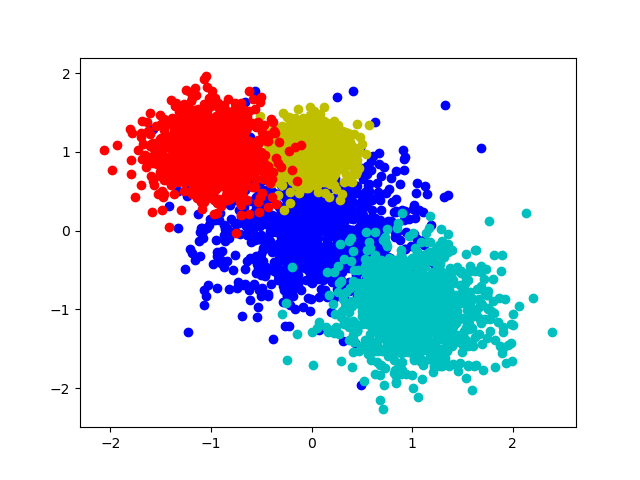
\includegraphics[width = .7\textwidth]{multi4.png}
  \caption{multiclass data points}
  \label{dataset}
\end{figure}

we explored SBM, BM, LBFGS, GD and SGD whose parameter settings are tuned and shown in $\ref{parameter}$

\begin{table}[htbp]
  \caption{parameter setting}
  \label{parameter}
  \centering
  \begin{tabular}{lllll}
    \toprule
    \multicolumn{5}{c}{$p:$ batch size $\quad$  $m:$ number of vectors in LBFGS }                   \\
    \cmidrule(r){1-5}
    BM     & SBM    & LBFGS & GD & SGD \\
    \midrule
    $\lambda = 1e-2$ &  $p = 40$  & $\eta:$ line search &$\lambda = 1e-2$ &$p = 40$      \\
     $\epsilon = 1e-6$    &  $\epsilon = 1e-6$  &  $\epsilon = 1e-5$ & $\epsilon = 1e-5$& $\epsilon = 1e-5$ \\
    $ \eta = 1$   &  $ \eta = 1e-2$   &  $m = 4$ &$\eta = 1e-2$ &$\eta = 1e-2$  \\
    \bottomrule
  \end{tabular}
\end{table}

The loglikelihood in the training procedure with respect to time and iteration were plotted, along with the training and testing error
with respect to the epoch. Just as what is shown in $\ref{loglikelihood}$ and $\ref{accuracy}$.

\begin{figure}[htbp]
  \centering
  \begin{subfigure}[b]{0.45\textwidth}
      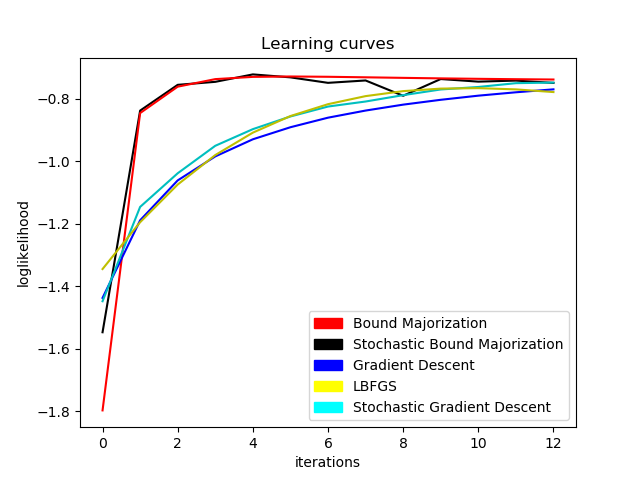
\includegraphics[width=\textwidth]{iterations}
      \caption{}
      \label{iteration}
  \end{subfigure}
  ~ %add desired spacing between images, e. g. ~, \quad, \qquad, \hfill etc. 
    %(or a blank line to force the subfigure onto a new line)
  \begin{subfigure}[b]{0.45\textwidth}
      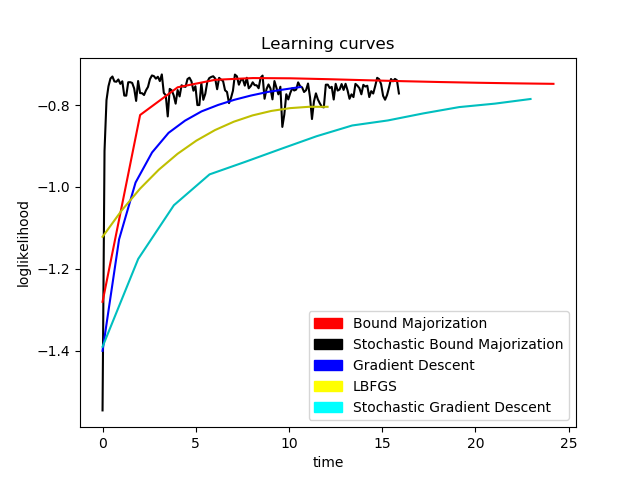
\includegraphics[width=\textwidth]{time}
      \caption{}
      \label{time}
  \end{subfigure}

  \caption{loglikelihood change}\label{loglikelihood}
\end{figure}

\begin{figure}[htbp]
  \centering
  \begin{subfigure}[b]{0.45\textwidth}
      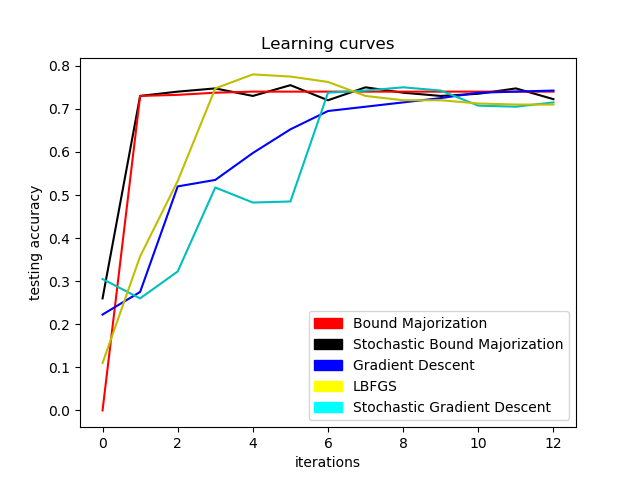
\includegraphics[width=\textwidth]{test_accuracy}
      \caption{}
      \label{test}
  \end{subfigure}
  ~ %add desired spacing between images, e. g. ~, \quad, \qquad, \hfill etc. 
    %(or a blank line to force the subfigure onto a new line)
  \begin{subfigure}[b]{0.45\textwidth}
      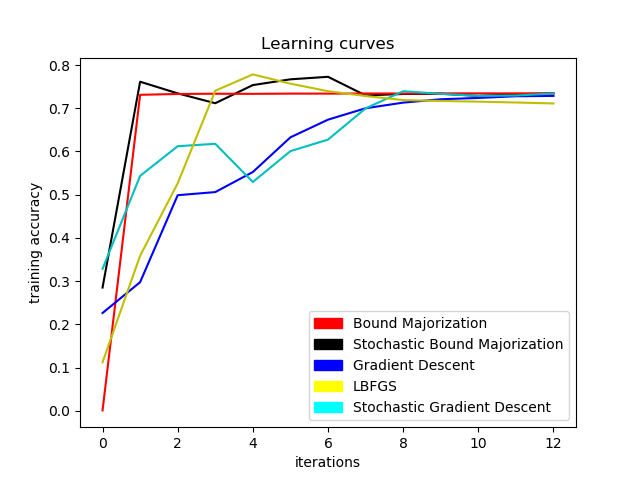
\includegraphics[width=\textwidth]{train_accuracy}
      \caption{}
      \label{train}
  \end{subfigure}

  \caption{training and testing accuracy}\label{accuracy}
\end{figure}
As can be seen clearly from the learning curves above, The BM algorithm and SBM algorithm surpassed others in convergence speed with respect to both time and
update epoch(where a single iteration corresponds to a single update of the parameter vector), while SBM requires much less time than any other algorithms. 

Note that 90$\%$ of the data is used for training and the rest for testing after randomly permuting the data,  
the results are averaged over 10-fold cross-validation, several values of $\lambda$ were explored and tuned.


\section{Conclusion}

Starting with interpretation of the log-linear partition model, the theoretical development of the algorithm has been revealed as a majorization procedure similiar to EM algorithm. Applying Sherman Morrison formula to 
 get $\ref{algorithm4}$ through which we can update without computing the matrix inverse, thus improving the efficiency.
 The convergence behavior was described not only in a sense of how many iteration is required under corresponding tolerance, but also in a sense of how close it would get to optimal after certain iterations,
 the proofs are given analogous to proving the statitiscal guarantee of stochastic EM, several assumptions were proposed without loss of generosity. 

 the proposed method, which requires no parameter tuning, has been evalueated as much more efficient than most of the first order methods such as LBFGS and SGD. The main drawbacks is that 
 it can only be applied to log-linear model, in the context of specific partition loss function which has the nice property to allow us find a simple quadratic bound. 







\section*{References}

\small

[1] Jebara, Tony, and Anna Choromanska. {\it"Majorization for CRFs and latent likelihoods."}
 {\it Advances in Neural Information Processing Systems.} 2012.

[2] Choromanska, Anna, and Tony Jebara. {\it"Stochastic bound majorization." arXiv preprint arXiv:1309.5605} (2013).

[3] T. Jebara. {\it Multitask sparsity via maximum entropy discrimination. JMLR, 12:75–110,} 2011.

\end{document}